\section{Dualshock4 Treiber (Becker)}

\subsection{Übertragung}

\subsection{Version 1: eigens entwickelter Treiber}

\subsection{Version 2: Treiber basierend auf der Bluepad32 Bibliothek}

\subsection{Testing}

\section{Platformsteuerung (Becker)}

Die sogenannte Plattformsteuerung bezeichnet alle technischen Komponenten, die erforderlich sind, um die Plattform in ihrer Rotation, vertikalen Neigung sowie für die Abgabe eines Schusses zu steuern.

Für den genannten Zweck werden folgende Komponenten benötigt:

\begin{itemize}
    \item \textbf{Drehung und Neigung}
    \begin{itemize}
        \item zwei MG996R Servo Motoren
    \end{itemize}
    \item \textbf{Schussabgabe}
    \begin{itemize}
        \item zwei DC-Motoren (Flywheels)
        \item MG92B Servo Motor
    \end{itemize}
\end{itemize}

Da die maximale Ausgangsstärke eines GPIO-PINs des ESP-32 mit 40mA \cite[S.~53]{esp_datasheet} für die benötigten Motoren nicht ausreicht \cite{esp_platform_flywheel_motor,esp_platform_small_servo,esp_platform_servo}, wurden entsprechende Treiberbaords verwendet.
Konkret handelt es sich hierbei um ein PCA9685 PWM-Treiberboard für die Servomotoren und um per PWM steuerbare MOSFET-Module für die Flywheel-Motoren.

In der nachfolgenden Sektion wird der Entwurf des Codes erörtert, der erforderlich ist, um die genannten Teile anzusteuern.

\subsection{PWM Board Treiber (Becker)}

Das PCA9685 PWM-Treiberboard gestattet die gleichzeitige Anbindung von bis zu 16 Servomotoren.
Für die Stromversorgung steht ein Eingang mit einer Spannung von 5 Volt zur Verfügung.

Die Steuerung des Boards erfolgt durch das Schreiben verschiedener Werte in Konfigurationsregister, wobei das I²C-Protokoll zum Einsatz kommt. 
Der vorliegende Treiber wurde aus der Portierung eines bereits bestehenden Treibers \cite{esp_pca9685_blueprint} entwickelt, welcher in der Programmiersprache C++ implementiert war. 
Es wurde bewusst nur die Funktionalität portiert, die für den Umfang des Projekts von Relevanz war. 
Der Treiber umfasst demzufolge lediglich drei Funktionen:

\begin{itemize}
    \item \textbf{pca9685\_init}: Die Funktion erhält die gewünschte Konfiguration für das Board (beispielsweise die Bus-Adresse, die SDA- und SCL-Ports für den I²C-Bus) und initialisiert den I²C-Bus. 
    Im Anschluss registriert sie das Treiberboard und konfiguriert schließlich das Board mit der gewünschten PWM-Frequenz.
    \item \textbf{pca9685\_set\_pwm\_on\_off}: Mithilfe dieser Funktion besteht nun die Möglichkeit, einen Motor auf einem der 16 Kanäle zu steuern. 
    Der Parameter \textit{ON} ist eine 12-Bit Zahl beschreibt hierbei den Zeitpunkt in der Phase, an welchem der Ausgang auf 5 Volt geschalten wird. 
    \textit{OFF}, ebenfalls eine 12-Bit Zahl bezeichnet den Zeitpunkt, zu welchem der Ausgang wieder auf 0 Volt geregelt wird. 
    Eine grafische Veranschaulichung ist in Abbildung \ref{fig:esp_pca9685_on_off} ersichtlich. 
    Da für die Ansteuerung der Servo Motoren keine symmetrischen PWM-Signale benötigt werden, wird der Parameter \textit{ON} im Folgenden immer den Wert 0 annehmen.

    \begin{figure}[ht]
        \centering
        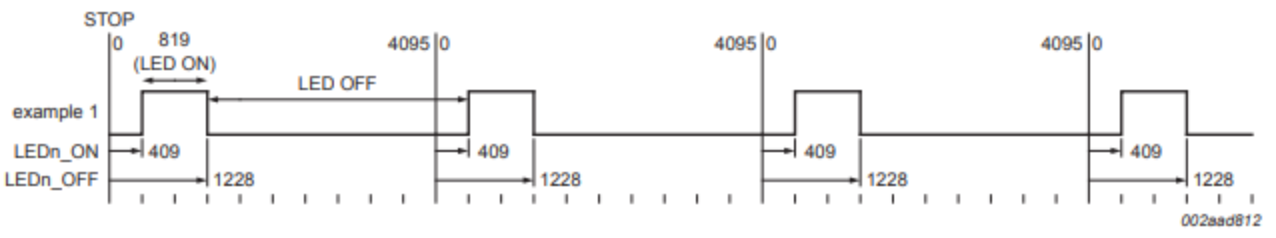
\includegraphics[width=\textwidth]{images/becker_esp_pca9685.png}
        \caption{Erklärung ON\slash OFF Parameter für PCA9685 aus \cite[S.~17]{esp_pca9685_datasheet}}
        \label{fig:esp_pca9685_on_off}
    \end{figure}

    \item \textbf{pca9685\_set\_off}: Mittels dieser Funktion kann das PWM-Signal auf einem bestimmten Kanal deaktiviert werden.
\end{itemize}

Auf Basis dieses Treiber wurden im nächsten Schritt zwei Interfaces programmiert: 
Einerseits das Interface zur Plattform-Kontrolle und andererseits das Interface zur Schusskontrolle, welches zusätzlich der Logik zur Ansteuerung der Flywheel-Motoren enthält.

\subsection{Ansteuerung der Servo-Motoren (Becker)}

Um nun die Plattform sowohl manuell über den DualShock4-Controller als auch semi-automatisch per künstlicher Intelligenz über MQTT präzise steuern zu können, wurde ein Interface entwickelt, das die Ansteuerung eines Motors an eine bestimmte Position erlaubt. 

In diesem Kontext wird mit der Einheit Grad gearbeitet. 
Ein Blick in die Referenz \cite{esp_servo_control} der Servo-Motoren zeigt, dass durch die Einstellung der Duty-Cycle-Länge des PWM-Signals eine Drehung auf eine bestimmte Grad-Position erreicht wird. 
Im ersten Schritt wurden die \textit{OFF} Werte für die Punkte \ang{-90} (max. Drehung nach links), \ang{0} und \ang{90} (max. Drehung nach rechts) manuell ermittelt.
Die absoluten Werte für die Drehungen werden im Folgenden als $value_{-90^\circ}$, $value_{0^\circ}$ und $value_{90^\circ}$ bezeichnet.

Für die Berechnung des Zielwerts $value_{off}$ für den \textit{OFF} Wert des PWM-Board-Treibers aus einem gegebenen Winkel wird Formel \ref{eq:pwm_to_duty} verwendet.

\begin{gather}
    \begin{aligned}
    &\text{Sei } \theta \text{ der gewünschte Winkel,} \\
    &|\theta| = \text{Betrag von } \theta \\
    &n_3 = \left\lfloor \frac{|\theta|}{3} \right\rfloor \\
    &n_2 = |\theta| - n_3 \\
    &s = 2 \cdot n_2 + 3 \cdot n_3 \\
    &\tilde{s} =
    \begin{cases}
    s, & \theta > 0 \\
    -s, & \theta \leq 0
    \end{cases} \\
    &value_{off} = value_{zero} + \tilde{s}
    \end{aligned}
    \label{eq:pwm_to_duty}
\end{gather}

Die Idee der Formel beruht auf der Tatsache, dass die Differenz aus $value_{90^\circ}$ bzw. $value_{-90^\circ}$ und $value_{0^\circ}$ gebildet und anschließend gleichmäßig auf den Bereich von $]1, 90[$, also auf 90 Werte, aufgeteilt wird. 

Für jedes zusätzliche Grad Rotation um den Nullpunkt müssten demnach entweder $2.\overline{3}$ addiert oder subtrahiert werden.
Da dies in Anbetracht der Verwendung von Festkommazahlen nicht realisierbar wäre, erscheint die naheliegende Idee, den Wert zu runden. 
Diese Praktik würde jedoch im Zeitverlauf zu einer zunehmenden Abweichung und folglich zu einem Verlust an Präzision führen.
Um das genannte Problem zu vermeiden, wird der \textit{OFF} Wert für jedes dritte Grad Drehung um den Faktor 3 verändert und für jedes andere Grad um Faktor 2.
Die Formel \ref{eq:pwm_to_duty} berechnet dabei in $n_3$ die Anzahl der Faktor-3-Drehungen und in $n_2$ die Anzahl der Faktor-2-Drehungen.
Ausgehend davon wird $value_{0^\circ}$ verändert.

Das Endergebnis stellt eine Funktion dar, mittels derer eine präzise gradweise Ansteuerung beider Plattformachsen möglich ist.

Darüber hinaus wurde im Interface ein Clipping der Werte als Sicherheitmechanismus integriert. Im Zuge der Initialisierung des Plattforminterfaces muss für jede Achse ein Startwinkel sowie ein linker und rechter Stopwinkel angegeben werden.
Sollte es bei der Steuerung durch den Dualshock4-Controller in dessen Regelschleife oder in der KI-Berechnung zu einem fehlerhaften Gradwert kommen, wird dieser Wert automatisch an den nächstgelegenen Stopwinkel geclippt. 
Durch diese Maßnahme werden potenzielle Materialschäden, die durch fehlerhafte Drehungen verursacht werden könnten, verhindert.

Die Realisierung der Ansteuerung des kleinen Servos, dessen Funktion darin besteht, die Nerf-Darts in die Flywheel-Motoren zu schieben, würde durch die Verwendung dieser Art der Ansteuerung zu einer unnötigen Komplexität führen.
Daher wurde für diesen Motor lediglich eine Startposition (Geschütztrigger ganz hinten; Dart kann in das Magazin fallen) und eine Endposition (Geschütztrigger ganz vorne; Dart wurde in die Flywheels geschoben) durch manuelles Einsetzen von \textit{OFF} Werten festgelegt.
Wird nun ein Schuss ausgelöst, so fährt der Servo-Motor zunächst in seine Endposition und von dort aus wieder zurück in seine Startposition.

\subsection{Ansteuerung der Flywheel Motoren (Becker, Koch, Wohlrab)}

Für die Vervollständigung des Fire-Control Interfaces wird nun noch die Ansteuerung der Flywheel-Motoren benötigt.
In dem vorliegenden Projekt erfolgt die Steuerung der beiden Gleichstrommotoren jeweils durch ein Power-MOSFET-Modul.

Die Funktionsweise des Modul lässt sich folgendermaßen beschreiben:

\begin{itemize}
    \item Auf einer Seite wird der Eingangstrom, in unserem Fall 5V, vom Stromverteiler eingeführt.
    \item Andererseits wird der Ausgang jeweils mit einem Motor verbunden.
    \item Die am Ausgang ausgegebene Spannung kann über einen PWM-Pin geregelt werden \cite{esp_platform_flywheel_motor}.
\end{itemize}

Die Wahl fiel auf dieses relativ simple Modul, da lediglich die Anforderung bestand, dass sich die Motoren bei der Schussabgabe möglichst schnell drehen sollen.
Im Rahmen dieses Projekts waren keine Änderungen der Richtung oder präzisere Steuerung erforderlich.

Im Rahmen des manuellen Tests wurde festgestellt, dass zur Erzielung eines optimalen Schussbildes eine Versorgung der Motoren mit 5 Volt erforderlich ist. 
Infolgedessen beträgt der Duty-Cycle entweder 0 oder 100 Prozent.
Daher wurde der ursprüngliche PWM-Code letztlich auf das reine Ein- und Ausschalten eines GPIO-Pins reduziert.

\section{Integration (Becker, Specht)}